% =============================================================================
% Chapter 3: System Design
% =============================================================================
% Required packages (add to your main preamble):
%   \usepackage{tikz}
%   \usetikzlibrary{shapes, arrows.meta, positioning, calc, fit}
%   \usepackage{algorithm}
%   \usepackage{algpseudocode}
%   \usepackage{booktabs}
%   \usepackage{amsmath}
% =============================================================================

\chapter{System Design}
\label{ch:design}

This chapter presents the architectural design of the multi-cluster Kubernetes resource sharing system. We first define the functional and non-functional requirements, then describe the overall architecture, data model, resource calculation, decision algorithm, communication protocol, security model, and the integration with Liqo for automatic cluster peering.


% =============================================================================
\section{Requirements}
\label{sec:requirements}

The system requirements are derived from the research objectives outlined in Chapter~\ref{ch:introduction} and the limitations identified in the state of the art (Chapter~\ref{ch:background}).

% -----------------------------------------------------------------------------
\subsection{Functional Requirements}
\label{subsec:functional-req}

\begin{enumerate}[label=\textbf{FR\arabic*}]
    \item \textbf{Resource Advertisement.}
    Each cluster must periodically collect its local resource metrics (CPU, memory, GPU) and publish them to the central broker. The advertisement must reflect real-time values including allocatable capacity, allocated resources, and any previously reserved quantities.

    \item \textbf{Advertisement Collection and Storage.}
    The broker must receive advertisements from all connected agents, store them as Kubernetes Custom Resources (\texttt{ClusterAdvertisement}), and maintain an up-to-date view of the entire federation's resource availability.

    \item \textbf{Reservation Processing.}
    When a user creates a reservation request specifying the desired CPU and memory, the broker must evaluate all available clusters through a decision engine and select the optimal provider.

    \item \textbf{Resource Locking.}
    Upon selecting a provider, the broker must atomically update the \texttt{Reserved} field in the provider's \texttt{ClusterAdvertisement} to prevent other reservations from consuming the same resources. This ensures consistency under concurrent requests.

    \item \textbf{Instruction Delivery.}
    After a successful reservation, the broker must generate two instruction objects: a \texttt{ReservationInstruction} for the requester (identifying the target provider) and a \texttt{ProviderInstruction} for the provider (identifying the requester and reserved quantities).

    \item \textbf{Automatic Cluster Peering.}
    Upon receiving a \texttt{ReservationInstruction}, the requester agent must automatically establish network-level peering with the provider cluster using Liqo, creating a virtual node that enables workload offloading.

    \item \textbf{Resource Release.}
    When a reservation expires or is explicitly released, the broker must unlock the reserved resources by updating the provider's \texttt{ClusterAdvertisement}, making those resources available for future reservations.
\end{enumerate}

% -----------------------------------------------------------------------------
\subsection{Non-Functional Requirements}
\label{subsec:nonfunctional-req}

\begin{enumerate}[label=\textbf{NFR\arabic*}]
    \item \textbf{Mutual TLS Security.}
    All communication between agents and the broker must be authenticated and encrypted using mutual TLS (mTLS). Each cluster's identity is derived from its client certificate Common Name (CN), eliminating the need for separate authentication tokens.

    \item \textbf{Scalability.}
    The system must support at least 20 simultaneously connected clusters with sub-second reservation latency. The broker's resource consumption must scale linearly with the number of connected agents.

    \item \textbf{Consistency Under Concurrency.}
    Multiple simultaneous reservation requests must be handled without double-booking resources. The \texttt{Reserved} field mechanism must guarantee that the same capacity is never allocated to more than one requester.

    \item \textbf{Lightweight Agent Footprint.}
    Individual agents must consume minimal resources (under 50~MB memory, under 5\% CPU) to allow deployment on resource-constrained edge nodes without impacting application workloads.

    \item \textbf{Protocol Extensibility.}
    The communication layer must be designed as a pluggable interface, allowing future transport protocols (e.g., MQTT, gRPC) to be added without modifying the core business logic.
\end{enumerate}


% =============================================================================
\section{Architecture Overview}
\label{sec:architecture}

The system follows a \textbf{hub-and-spoke} architecture where a central broker coordinates resource sharing among multiple Kubernetes clusters. Each cluster runs an agent that communicates with the broker via HTTPS with mutual TLS authentication. Figure~\ref{fig:architecture} illustrates the high-level architecture.

\begin{figure}[htbp]
\centering
\begin{tikzpicture}[
    node distance=1.5cm,
    component/.style={rectangle, draw, rounded corners, minimum width=2.8cm, minimum height=0.7cm, font=\small},
    cluster/.style={rectangle, draw, thick, rounded corners=8pt, minimum width=5cm, minimum height=5.5cm, fill=white},
    arrow/.style={-{Stealth[length=2.5mm]}, thick},
    doublearrow/.style={{Stealth[length=2.5mm]}-{Stealth[length=2.5mm]}, thick, double, double distance=1.5pt},
    label/.style={font=\footnotesize\itshape},
]

% Broker cluster
\node[cluster, fill=blue!5] (broker) {};
\node[font=\bfseries\small, anchor=north] at (broker.north) {Broker Cluster};
\node[component, fill=blue!15] (api) at ([yshift=-0.8cm]broker.north) {REST API (mTLS)};
\node[component, fill=blue!15, below=0.3cm of api] (decision) {Decision Engine};
\node[component, fill=blue!15, below=0.3cm of decision] (cadvs) {ClusterAdvertisements};
\node[component, fill=blue!15, below=0.3cm of cadvs] (reservations) {Reservations};

% Agent cluster 1 (left)
\node[cluster, fill=green!5, left=3cm of broker] (agent1) {};
\node[font=\bfseries\small, anchor=north] at (agent1.north) {Agent Cluster (Requester)};
\node[component, fill=green!15] (collector1) at ([yshift=-0.8cm]agent1.north) {Metrics Collector};
\node[component, fill=green!15, below=0.3cm of collector1] (adv1) {Advertisement};
\node[component, fill=green!15, below=0.3cm of adv1] (ri) {ReservationInstruction};
\node[component, fill=green!15, below=0.3cm of ri] (liqo1) {Liqo Peering};

% Agent cluster 2 (right)
\node[cluster, fill=orange!5, right=3cm of broker] (agent2) {};
\node[font=\bfseries\small, anchor=north] at (agent2.north) {Agent Cluster (Provider)};
\node[component, fill=orange!15] (collector2) at ([yshift=-0.8cm]agent2.north) {Metrics Collector};
\node[component, fill=orange!15, below=0.3cm of collector2] (adv2) {Advertisement};
\node[component, fill=orange!15, below=0.3cm of adv2] (pi) {ProviderInstruction};
\node[component, fill=orange!15, below=0.3cm of pi] (liqo2) {Liqo};

% Virtual node
\node[component, fill=green!30, dashed, below=0.3cm of liqo1, minimum width=2.6cm] (vnode) {\footnotesize Virtual Node};

% Arrows: Agent 1 <-> Broker
\draw[arrow, color=blue!60] (adv1.east) -- node[above, label] {HTTPS/mTLS} (api.west);
\draw[arrow, color=blue!60, dashed] (api.west) -- +(-0.5,0) |- (ri.east);

% Arrows: Agent 2 <-> Broker
\draw[arrow, color=orange!60] (adv2.west) -- node[above, label] {HTTPS/mTLS} (api.east);
\draw[arrow, color=orange!60, dashed] (api.east) -- +(0.5,0) |- (pi.west);

% Liqo peering arrow
\draw[doublearrow, color=purple!60] (liqo1.east) -- node[below, label, yshift=-2pt] {Liqo Peering} node[above, label, yshift=2pt] {\footnotesize (WireGuard)} (liqo2.west);

\end{tikzpicture}
\caption{System architecture. Agents publish resource advertisements to the broker via HTTPS/mTLS. The broker processes reservations and delivers instructions. The requester agent automatically peers with the provider via Liqo.}
\label{fig:architecture}
\end{figure}

% -----------------------------------------------------------------------------
\subsection{Broker Component}
\label{subsec:broker-design}

The broker is the central coordination point of the system, deployed as a Kubernetes controller-manager within its own cluster. It exposes a REST API server secured with mutual TLS and manages the following responsibilities:

\begin{itemize}
    \item \textbf{Advertisement reception:} Receives and stores resource advertisements from all connected agents as \texttt{ClusterAdvertisement} Custom Resources.
    \item \textbf{Reservation processing:} When a \texttt{Reservation} is created, the broker's controller invokes the decision engine to select the best provider cluster.
    \item \textbf{Resource locking:} Updates the \texttt{Reserved} field in the selected provider's advertisement to prevent double-booking.
    \item \textbf{Instruction generation:} Returns \texttt{ReservationInstruction} and \texttt{ProviderInstruction} objects when agents poll for new reservations.
    \item \textbf{Score calculation:} Computes and maintains a score for each cluster advertisement based on resource availability.
\end{itemize}

% -----------------------------------------------------------------------------
\subsection{Agent Component}
\label{subsec:agent-design}

The agent is deployed in each participating cluster and operates as a Kubernetes operator. It performs the following functions:

\begin{itemize}
    \item \textbf{Resource collection:} Monitors local nodes and pods to calculate CPU, memory, and GPU availability using the formula defined in Section~\ref{sec:resource-calculation}.
    \item \textbf{Advertisement publishing:} Periodically sends the collected metrics to the broker, preserving the \texttt{Reserved} field set by the broker to avoid overwriting locked resources.
    \item \textbf{Reservation polling:} Queries the broker for pending reservations involving this cluster, either as requester or provider.
    \item \textbf{Instruction management:} Creates local \texttt{ReservationInstruction} or \texttt{ProviderInstruction} CRDs based on broker responses.
    \item \textbf{Liqo peering:} When a \texttt{ReservationInstruction} is received, the agent automatically triggers \texttt{liqoctl peer} to establish network peering with the provider cluster.
\end{itemize}


% =============================================================================
\section{Data Model}
\label{sec:data-model}

The system uses Kubernetes Custom Resource Definitions (CRDs) as its primary data model. CRDs extend the Kubernetes API with application-specific resource types, allowing the system to leverage Kubernetes' built-in reconciliation, watch mechanisms, and RBAC. Figure~\ref{fig:data-model} shows the relationships between the CRDs.

\begin{figure}[htbp]
\centering
\begin{tikzpicture}[
    node distance=2cm,
    crd/.style={rectangle, draw, thick, rounded corners, minimum width=4.5cm, minimum height=1cm, font=\small\bfseries},
    field/.style={rectangle, draw, minimum width=4.5cm, font=\footnotesize, anchor=north},
    arrow/.style={-{Stealth[length=2.5mm]}, thick},
]

% Broker-side CRDs
\node[crd, fill=blue!15] (cadv) {ClusterAdvertisement};
\node[crd, fill=blue!15, right=3cm of cadv] (res) {Reservation};

% Agent-side CRDs
\node[crd, fill=green!15, below=3cm of cadv] (ri) {ReservationInstruction};
\node[crd, fill=orange!15, below=3cm of res] (pi) {ProviderInstruction};
\node[crd, fill=gray!15, left=3cm of cadv] (adv) {Advertisement};

% Arrows
\draw[arrow] (adv) -- node[above, font=\footnotesize\itshape] {publishes to} (cadv);
\draw[arrow] (res) -- node[right, font=\footnotesize\itshape, align=center] {locks resources\\in} (cadv);
\draw[arrow] (res) -- node[right, font=\footnotesize\itshape, align=center] {generates} (pi);
\draw[arrow] (res) -- node[left, font=\footnotesize\itshape, align=center] {generates} (ri);

% Labels
\node[font=\footnotesize\itshape, below=0.1cm of adv] {(Agent cluster)};
\node[font=\footnotesize\itshape, below=0.1cm of cadv] {(Broker cluster)};
\node[font=\footnotesize\itshape, below=0.1cm of res] {(Broker cluster)};
\node[font=\footnotesize\itshape, below=0.1cm of ri] {(Requester cluster)};
\node[font=\footnotesize\itshape, below=0.1cm of pi] {(Provider cluster)};

\end{tikzpicture}
\caption{CRD relationships. The agent's local Advertisement is published to the broker as a ClusterAdvertisement. Reservations lock resources in the advertisement and generate instructions for both sides.}
\label{fig:data-model}
\end{figure}

% -----------------------------------------------------------------------------
\subsection{ClusterAdvertisement}
\label{subsec:cluster-adv}

The \texttt{ClusterAdvertisement} CRD resides in the broker cluster and represents the resource state of a remote cluster. Table~\ref{tab:cluster-adv} lists the specification fields.

\begin{table}[htbp]
\centering
\caption{\texttt{ClusterAdvertisement} specification fields}
\label{tab:cluster-adv}
\begin{tabular}{@{}llp{7cm}@{}}
\toprule
\textbf{Field} & \textbf{Type} & \textbf{Description} \\
\midrule
\texttt{clusterID} & string & Unique identifier for the cluster \\
\texttt{resources.capacity} & ResourceQuantities & Total physical resources of all nodes \\
\texttt{resources.allocatable} & ResourceQuantities & Capacity minus system-reserved resources \\
\texttt{resources.allocated} & ResourceQuantities & Sum of all running pod resource requests \\
\texttt{resources.reserved} & ResourceQuantities & Resources locked by broker reservations \\
\texttt{resources.available} & ResourceQuantities & Computed: allocatable $-$ allocated $-$ reserved \\
\texttt{timestamp} & Time & Last update timestamp \\
\texttt{cost} & CostInfo & Optional cost per CPU/memory unit \\
\bottomrule
\end{tabular}
\end{table}

Each \texttt{ResourceQuantities} struct contains \texttt{cpu} (in millicores), \texttt{memory} (in bytes), and optionally \texttt{gpu} and \texttt{storage} fields, all using Kubernetes' standard \texttt{resource.Quantity} type.

The status fields include:

\begin{table}[htbp]
\centering
\caption{\texttt{ClusterAdvertisement} status fields}
\label{tab:cluster-adv-status}
\begin{tabular}{@{}llp{7cm}@{}}
\toprule
\textbf{Field} & \textbf{Type} & \textbf{Description} \\
\midrule
\texttt{active} & bool & Whether the cluster is available for reservations \\
\texttt{score} & string & Computed availability score (0--100) \\
\texttt{lastUpdateTime} & Time & Timestamp of last status change \\
\texttt{conditions} & []Condition & Ready, Stale, or Overcommitted \\
\bottomrule
\end{tabular}
\end{table}

% -----------------------------------------------------------------------------
\subsection{Reservation}
\label{subsec:reservation}

The \texttt{Reservation} CRD represents a resource request. Table~\ref{tab:reservation} lists its fields.

\begin{table}[htbp]
\centering
\caption{\texttt{Reservation} specification fields}
\label{tab:reservation}
\begin{tabular}{@{}llp{7cm}@{}}
\toprule
\textbf{Field} & \textbf{Type} & \textbf{Description} \\
\midrule
\texttt{requesterID} & string & Cluster ID of the requesting agent \\
\texttt{targetClusterID} & string & Auto-selected by broker (or manually specified) \\
\texttt{requestedResources.cpu} & Quantity & Requested CPU (e.g., ``500m'') \\
\texttt{requestedResources.memory} & Quantity & Requested memory (e.g., ``256Mi'') \\
\texttt{priority} & int32 & Higher values indicate higher priority \\
\texttt{duration} & Duration & Optional reservation time limit \\
\bottomrule
\end{tabular}
\end{table}

A reservation progresses through a well-defined lifecycle, as shown in Figure~\ref{fig:reservation-lifecycle}.

\begin{figure}[htbp]
\centering
\begin{tikzpicture}[
    node distance=2.5cm,
    state/.style={circle, draw, thick, minimum size=1.5cm, font=\small\bfseries, inner sep=2pt},
    arrow/.style={-{Stealth[length=2.5mm]}, thick},
]

\node[state, fill=yellow!20] (pending) {Pending};
\node[state, fill=green!20, right=of pending] (reserved) {Reserved};
\node[state, fill=blue!20, right=of reserved] (active) {Active};
\node[state, fill=gray!20, right=of active] (released) {Released};
\node[state, fill=red!20, below=1.5cm of reserved] (failed) {Failed};

\draw[arrow] (pending) -- node[above, font=\footnotesize] {provider selected} (reserved);
\draw[arrow] (reserved) -- node[above, font=\footnotesize] {agent confirms} (active);
\draw[arrow] (active) -- node[above, font=\footnotesize] {released/expired} (released);
\draw[arrow] (pending) -- node[left, font=\footnotesize, align=center] {no suitable\\cluster} (failed);
\draw[arrow] (reserved) -- node[right, font=\footnotesize] {expired} (released);

\end{tikzpicture}
\caption{Reservation lifecycle. A reservation transitions from Pending through Reserved and Active to Released. If no suitable provider is found, it transitions to Failed.}
\label{fig:reservation-lifecycle}
\end{figure}

% -----------------------------------------------------------------------------
\subsection{Instructions}
\label{subsec:instructions}

After a reservation reaches the \textit{Reserved} phase, the system generates two instruction CRDs to notify the involved clusters.

\textbf{ReservationInstruction} is created in the requester's cluster:

\begin{table}[htbp]
\centering
\caption{\texttt{ReservationInstruction} fields}
\label{tab:reservation-instruction}
\begin{tabular}{@{}llp{7cm}@{}}
\toprule
\textbf{Field} & \textbf{Type} & \textbf{Description} \\
\midrule
\texttt{reservationName} & string & Reference to the broker-side Reservation \\
\texttt{targetClusterID} & string & Provider cluster to peer with \\
\texttt{requestedCPU} & string & CPU quantity granted \\
\texttt{requestedMemory} & string & Memory quantity granted \\
\texttt{expiresAt} & Time & Reservation expiration time \\
\texttt{status.delivered} & bool & Whether Liqo peering was initiated \\
\bottomrule
\end{tabular}
\end{table}

\textbf{ProviderInstruction} is created in the provider's cluster:

\begin{table}[htbp]
\centering
\caption{\texttt{ProviderInstruction} fields}
\label{tab:provider-instruction}
\begin{tabular}{@{}llp{7cm}@{}}
\toprule
\textbf{Field} & \textbf{Type} & \textbf{Description} \\
\midrule
\texttt{reservationName} & string & Reference to the broker-side Reservation \\
\texttt{requesterClusterID} & string & Cluster receiving the resources \\
\texttt{requestedCPU} & string & CPU quantity to reserve \\
\texttt{requestedMemory} & string & Memory quantity to reserve \\
\texttt{expiresAt} & Time & Reservation expiration time \\
\texttt{status.enforced} & bool & Whether the provider acknowledged the instruction \\
\bottomrule
\end{tabular}
\end{table}


% =============================================================================
\section{Resource Calculation}
\label{sec:resource-calculation}

A central challenge in multi-cluster resource sharing is maintaining an accurate view of each cluster's available capacity. The system uses the following formula to compute availability:

\begin{equation}
\label{eq:available}
\text{Available} = \text{Allocatable} - \text{Allocated} - \text{Reserved}
\end{equation}

\noindent where:

\begin{itemize}
    \item \textbf{Allocatable} is the sum of all ready nodes' allocatable resources. This equals the node's total capacity minus resources reserved by the operating system and Kubernetes system components (kubelet, kube-proxy, etc.).
    \item \textbf{Allocated} is the sum of all running and pending pods' resource \emph{requests} (not limits). Init containers are handled separately: their resources are not summed but the maximum across all init containers is taken, since they run sequentially.
    \item \textbf{Reserved} is the sum of all active \texttt{ProviderInstruction} resources that have been enforced and have not yet expired. This represents capacity locked by the broker for other clusters' reservations.
\end{itemize}

The \texttt{Reserved} field is the key mechanism for preventing race conditions. When the broker selects a provider for a reservation, it atomically increments the provider's \texttt{Reserved} field. Subsequent reservation decisions see the reduced available capacity, ensuring that the same resources are never double-booked. Figure~\ref{fig:resource-calculation} illustrates this visually.

\begin{figure}[htbp]
\centering
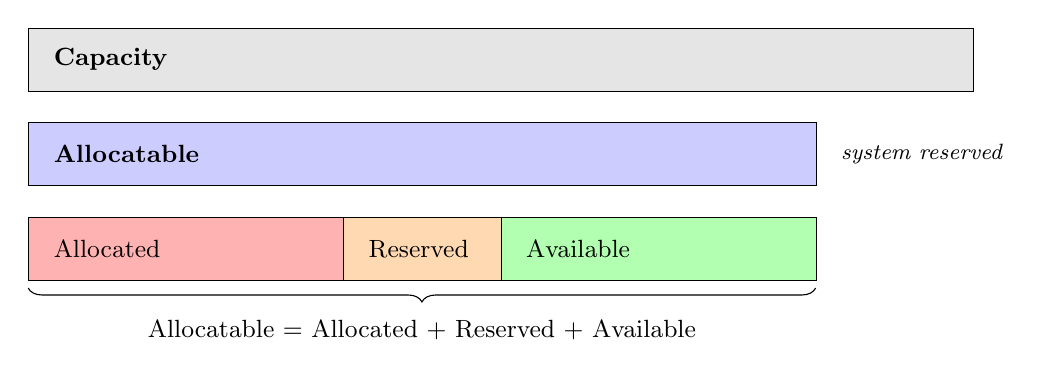
\begin{tikzpicture}[
    bar/.style={draw, minimum height=0.8cm, font=\small},
]
% Total bar
\node[bar, fill=gray!20, minimum width=12cm, anchor=west] (total) at (0,0) {};
\node[font=\small\bfseries, anchor=west] at (0.2, 0) {Capacity};

% Allocatable
\node[bar, fill=blue!20, minimum width=10cm, anchor=west] (alloc) at (0,-1.2) {};
\node[font=\small\bfseries, anchor=west] at (0.2, -1.2) {Allocatable};
\node[font=\footnotesize, anchor=west] at (10.2, -1.2) {\textit{system reserved}};

% Breakdown
\node[bar, fill=red!30, minimum width=4cm, anchor=west] (allocated) at (0,-2.4) {};
\node[font=\small, anchor=west] at (0.2, -2.4) {Allocated};

\node[bar, fill=orange!30, minimum width=2cm, anchor=west] (reserved) at (4,-2.4) {};
\node[font=\small, anchor=west] at (4.2, -2.4) {Reserved};

\node[bar, fill=green!30, minimum width=4cm, anchor=west] (available) at (6,-2.4) {};
\node[font=\small, anchor=west] at (6.2, -2.4) {Available};

% Braces
\draw[decorate, decoration={brace, amplitude=5pt, mirror}] (0,-2.9) -- (10,-2.9) node[midway, below=8pt, font=\small] {Allocatable = Allocated + Reserved + Available};

\end{tikzpicture}
\caption{Resource breakdown. Available capacity is what remains after subtracting allocated (running pods) and reserved (broker-locked) resources from the allocatable total.}
\label{fig:resource-calculation}
\end{figure}


% =============================================================================
\section{Decision Algorithm}
\label{sec:decision-algorithm}

The broker's decision engine selects the optimal provider cluster for each reservation request. The algorithm operates in three phases: \textit{filter}, \textit{score}, and \textit{select}.

\subsection{Filtering}

A cluster is excluded from consideration if any of the following conditions hold:
\begin{itemize}
    \item Its \texttt{clusterID} equals the requester's ID (a cluster cannot borrow from itself).
    \item Its \texttt{status.active} flag is \texttt{false} (the cluster is offline or stale).
    \item Its available CPU or memory is less than the requested quantities.
\end{itemize}

\subsection{Scoring}

Each remaining candidate cluster is assigned a score based on the \emph{remaining capacity after fulfillment}. The scoring formula is:

\begin{equation}
\label{eq:cpu-util}
U_{\text{cpu}} = 1 - \frac{\text{Available}_{\text{cpu}} - \text{Requested}_{\text{cpu}}}{\text{Allocatable}_{\text{cpu}}}
\end{equation}

\begin{equation}
\label{eq:mem-util}
U_{\text{mem}} = 1 - \frac{\text{Available}_{\text{mem}} - \text{Requested}_{\text{mem}}}{\text{Allocatable}_{\text{mem}}}
\end{equation}

\begin{equation}
\label{eq:score}
\text{Score} = \left(1 - 0.5 \cdot U_{\text{cpu}}\right) + \left(1 - 0.5 \cdot U_{\text{mem}}\right)
\end{equation}

\noindent where $U_{\text{cpu}}$ and $U_{\text{mem}}$ represent the projected utilization \emph{after} fulfilling the request. Lower utilization results in a higher score, meaning the algorithm favors clusters that would retain the most headroom after the reservation. This strategy distributes load across the federation and avoids concentrating reservations on a single cluster.

An optional cost penalty (multiplying the score by 0.9 if cost metadata is present) and a priority bonus ($\text{priority} \times 0.01$) are also applied.

\subsection{Selection}

The cluster with the highest score is selected as the provider. Algorithm~\ref{alg:decision} summarizes the complete procedure.

\begin{algorithm}[htbp]
\caption{Cluster Selection Algorithm}
\label{alg:decision}
\begin{algorithmic}[1]
\Require Set of ClusterAdvertisements $C$, requester ID $r$, requested CPU $q_c$, requested memory $q_m$, priority $p$
\Ensure Selected cluster $c^*$ or failure
\State $\text{bestScore} \gets -1$
\State $c^* \gets \text{nil}$
\ForAll{$c \in C$}
    \If{$c.\text{clusterID} = r$} \textbf{continue} \Comment{Skip self}
    \EndIf
    \If{$c.\text{active} = \text{false}$} \textbf{continue} \Comment{Skip inactive}
    \EndIf
    \If{$c.\text{available.cpu} < q_c$ \textbf{or} $c.\text{available.memory} < q_m$}
        \textbf{continue} \Comment{Skip insufficient}
    \EndIf
    \State $U_c \gets 1 - (c.\text{available.cpu} - q_c) / c.\text{allocatable.cpu}$
    \State $U_m \gets 1 - (c.\text{available.mem} - q_m) / c.\text{allocatable.mem}$
    \State $s \gets (1 - 0.5 \cdot U_c) + (1 - 0.5 \cdot U_m) + p \cdot 0.01$
    \If{$s > \text{bestScore}$}
        \State $\text{bestScore} \gets s$
        \State $c^* \gets c$
    \EndIf
\EndFor
\If{$c^* = \text{nil}$}
    \State \Return \textsc{Failed} \Comment{No suitable cluster found}
\EndIf
\State \Return $c^*$
\end{algorithmic}
\end{algorithm}


% =============================================================================
\section{Communication Protocol}
\label{sec:protocol}

The broker exposes a REST API over HTTPS. Table~\ref{tab:api-endpoints} lists the available endpoints.

\begin{table}[htbp]
\centering
\caption{Broker REST API endpoints}
\label{tab:api-endpoints}
\begin{tabular}{@{}llp{6.5cm}@{}}
\toprule
\textbf{Method} & \textbf{Endpoint} & \textbf{Description} \\
\midrule
\texttt{POST} & \texttt{/api/v1/advertisements} & Submit or update a cluster advertisement. The broker preserves the \texttt{Reserved} field. \\
\texttt{GET} & \texttt{/api/v1/advertisements/\{id\}} & Retrieve a specific cluster's advertisement (including the \texttt{Reserved} field set by the broker). \\
\texttt{GET} & \texttt{/api/v1/reservations} & Poll for reservations. Query parameters: \texttt{clusterID} and \texttt{role} (\texttt{requester} or \texttt{provider}). \\
\texttt{GET} & \texttt{/healthz} & Health check endpoint (no authentication required). \\
\bottomrule
\end{tabular}
\end{table}

The agent-broker interaction follows a \textbf{poll-based} model. Agents periodically publish their advertisement (every 10--30 seconds) and simultaneously poll for new reservations. This design avoids the need for the broker to maintain persistent connections or push notifications, simplifying deployment and firewall configuration.

Figure~\ref{fig:sequence} shows the complete reservation flow.

\begin{figure}[htbp]
\centering
\begin{tikzpicture}[
    font=\small,
    actor/.style={rectangle, draw, thick, minimum width=2.5cm, minimum height=0.8cm, font=\small\bfseries, fill=#1},
    arrow/.style={-{Stealth[length=2mm]}, thick},
    dashedarrow/.style={-{Stealth[length=2mm]}, thick, dashed},
    note/.style={font=\footnotesize\itshape},
]

% Actors
\node[actor=green!15] (a1) at (0, 0) {Agent 1};
\node[actor=blue!15] (broker) at (5.5, 0) {Broker};
\node[actor=orange!15] (a2) at (11, 0) {Agent 2};

% Lifelines
\draw[gray, thin] (0, -0.4) -- (0, -11);
\draw[gray, thin] (5.5, -0.4) -- (5.5, -11);
\draw[gray, thin] (11, -0.4) -- (11, -11);

% Step 1: Publish advertisements
\draw[arrow, blue!60] (0, -1) -- node[above, note] {POST /advertisements} (5.5, -1);
\draw[arrow, orange!60] (11, -1.5) -- node[above, note] {POST /advertisements} (5.5, -1.5);
\node[note, anchor=east] at (-0.3, -1.25) {1. Publish};

% Step 2: Create reservation
\node[note, anchor=east] at (-0.3, -2.5) {2. User creates};
\node[note, anchor=west] at (5.8, -2.5) {Reservation created};

% Step 3: Decision
\node[rectangle, draw, fill=blue!10, font=\footnotesize, inner sep=3pt] at (5.5, -3.5) {Decision Engine};
\node[note, anchor=east] at (-0.3, -3.5) {3. Select provider};

% Step 4: Lock resources
\node[note, anchor=east] at (-0.3, -4.5) {4. Lock resources};
\node[note, anchor=west] at (5.8, -4.5) {Reserved += requested};

% Step 5: Poll + instructions
\draw[arrow, blue!60] (0, -5.5) -- node[above, note] {GET /reservations?role=requester} (5.5, -5.5);
\draw[dashedarrow, blue!60] (5.5, -6) -- node[above, note] {ReservationInstruction} (0, -6);
\node[note, anchor=east] at (-0.3, -5.75) {5. Poll};

\draw[arrow, orange!60] (11, -6.5) -- node[above, note] {GET /reservations?role=provider} (5.5, -6.5);
\draw[dashedarrow, orange!60] (5.5, -7) -- node[above, note] {ProviderInstruction} (11, -7);

% Step 6: Liqo peering
\draw[arrow, purple!60, double, double distance=1pt] (0, -8.5) -- node[above, note] {liqoctl peer (WireGuard)} (11, -8.5);
\node[note, anchor=east] at (-0.3, -8.5) {6. Auto-peer};

% Step 7: Virtual node
\node[rectangle, draw, dashed, fill=green!10, font=\footnotesize, inner sep=3pt] at (0, -9.5) {Virtual Node created};
\node[note, anchor=east] at (-0.3, -9.5) {7. Offload ready};

\end{tikzpicture}
\caption{Reservation flow sequence. Numbers indicate the order of operations from advertisement publishing through Liqo peering.}
\label{fig:sequence}
\end{figure}


% =============================================================================
\section{Security Model}
\label{sec:security}

The system uses \textbf{mutual TLS (mTLS)} for all agent-broker communication. In mTLS, both the client (agent) and the server (broker) present certificates signed by a common Certificate Authority (CA), providing bidirectional authentication.

\subsection{Certificate Management}

Certificates are managed by \texttt{cert-manager}~\cite{cert-manager}, a Kubernetes-native certificate lifecycle manager deployed in the broker cluster. The CA hierarchy is:

\begin{enumerate}
    \item A self-signed \texttt{ClusterIssuer} creates the root CA.
    \item The root CA issues a server certificate for the broker (CN = \texttt{liqo-resource-broker}).
    \item The root CA issues a client certificate for each agent (CN = cluster ID, e.g., \texttt{agent-cluster-1}).
\end{enumerate}

\subsection{Identity Extraction}

The broker extracts the cluster identity from the client certificate's Common Name (CN) field using a middleware layer. This eliminates the need for API keys, tokens, or session management:

\begin{equation*}
    \text{ClusterID} = \text{Certificate.Subject.CN}
\end{equation*}

When an agent with CN = \texttt{agent-cluster-1} publishes an advertisement claiming \texttt{clusterID: agent-cluster-1}, the middleware verifies that the certificate CN matches the claimed identity, preventing impersonation.

\subsection{TLS Configuration}

The broker's TLS configuration enforces:
\begin{itemize}
    \item TLS 1.2 as the minimum protocol version.
    \item \texttt{RequireAndVerifyClientCert} policy, rejecting connections without valid client certificates.
    \item The \texttt{/healthz} endpoint is exempted from client certificate requirements to support load balancer health probes.
\end{itemize}


% =============================================================================
\section{Liqo Integration}
\label{sec:liqo-integration}

While the broker handles resource \emph{decision-making}, the actual cluster interconnection is delegated to Liqo~\cite{liqo}. After the broker assigns a provider to a requester, the requester's agent automatically establishes Liqo peering.

\subsection{Peering Trigger}

The \texttt{ReservationInstructionReconciler} in the agent monitors for new \texttt{ReservationInstruction} resources. When one appears with \texttt{delivered = false}, the controller:

\begin{enumerate}
    \item Locates the local and remote kubeconfig files based on the cluster IDs.
    \item Executes \texttt{liqoctl peer --kubeconfig <local> --remote-kubeconfig <remote> --gw-server-service-type NodePort}.
    \item Waits for the peering to complete (up to 5 minutes).
    \item Marks the instruction as \texttt{delivered = true}.
\end{enumerate}

\subsection{Virtual Node}

Upon successful peering, Liqo creates a \textbf{virtual node} in the requester's cluster. This virtual node appears alongside the physical nodes and advertises the resources available from the provider cluster. Standard Kubernetes scheduling can then place pods on the virtual node, which Liqo transparently offloads to the provider cluster via an encrypted WireGuard tunnel.

This approach preserves the standard Kubernetes abstraction: from the user's perspective, the provider's resources appear as a regular node, and no changes to existing deployment manifests are required.
